%===================================================================================
% Chapter: Marco Experimental
%===================================================================================

\chapter{Experimentación y Resultados} 
El objetivo de este capítulo es realizar la validación de la metodología que se presentó en este estudio se conformaron tres experimentos. El primero pretende estimar el número de clústeres óptimo para Kmeans, un parámetro sumamente importante para alcanzar buenos resultados. El segundo plantea una comparación entre el método de trayectorias simples y el método de trayectorias con las modificaciones propuestas. Por último, se diseñó un experimento a modo de comparación entre los algoritmos: Kmeas y Trayectorias Simples Modificado.
Los datos sobre los que se ejecutan los experimentos son descritos en el siguiente epígrafe. Para la realización de estas pruebas se utiliza una máquina con las siguientes características: Intel i7-660U,16 gb RAM.

\section{Datos}
Un aspecto fundamental en el estudio de la segregación es el procesamiento de los datos. Un análisis concreto de los mismos brinda información más que necesaria en base a criterios rigurosos que pueden influir en la toma de decisiones a la hora de determinar la existencia o no de segregación en un territorio o población determinada. Para la detección de la segregación en la Habana, se cuenta con datos provenientes de dos fuentes fundamentales: Oficina Nacional de Estadísticas e Información de la República de Cuba (ONEI) y el grupo empresarial GEOCUBA. De la ONEI se obtuvo el censo poblacional realizado en el 2012, que aporta un gran número de características y variables para realizar un análisis profundo sobre la población y la vivienda en la Habana. De GeoCuba se adquirió una base de datos que contiene datos geoespaciales para cada entidad del estudio.

Lograr establecer una relación entre ambas fuentes de datos no fue una tarea sencilla. Para encontrar un punto común entre ambas fuentes, se decidió asociar los datos en torno a distritos (conjunto de manzanas), que serán la unidad básica de medida en el estudio de segregación para ambos algoritmos. Vale destacar que, aunque la mayor parte de estudios poblacionales realizados en Cuba utilizan las circunscripciones como unidad base, la elección de los distritos no resulta una elección aleatoria. Por una parte, no se disponía de la ubicación geoespacial para las circunscripciones, unido a que los antecedentes a este trabajo, están realizados sobre la ciudad de Paris, lugar donde se toma con unidad base los IRIS. Un Iris es equivalente a la unión de varios distritos. 

La información referente al censo poblacional de la ONEI se reagrupó en torno a los distritos de cada municipio, obteniendo un cúmulo de variables muy importantes para el análisis; entre ellas: la cantidad de viviendas, la cantidad de población, clasificaciones de la población en cuanto al sexo, color y grupos de edades, por solo mencionar unas pocas. Este estudio se enfoca en el análisis de la variable “Edad de las viviendas”, pero el trabajo realizado abre las puertas al grupo de investigación para el análisis del resto de las variables en futuros trabajos. La geolocalización de los distritos presentó desafíos interesantes pues la base de datos de GEOCUBA tiene como unidad básica las manzanas. Para poder estimar la ubicación de los distritos fue necesario el siguiente análisis: en todo municipio existen múltiples distritos, los que a su vez están formados por múltiples manzanas, o sea, que si para cada distrito en un determinado municipio se cuenta con la geolocalización de cada una de las manzanas que pertenecen al mismo se puede aproximar su ubicación. Lo descrito anteriormente se realizó de la siguiente forma:
\begin{itemize}
	\item De los datos de la ONEI determinar el municipio del distrito.
	\item De los datos de la ONEI seleccionar todas las manzanas que forman parte del distrito.
	\item Para cada manzana perteneciente a dicho distrito buscar sus posibles coordenadas en la base de datos de GEOCUBA, recordar que para un mismo identificador de manzana en la base de datos de GEOCUBA existen varias entradas.
	\item Con todas las posibles coordenadas para una determinada manzana seleccionar aquella que pertenezca al municipio en cuestión, es necesario destacar que la pertenencia se tomó parcialmente pues los polígonos asociados a manzanas y los polígonos asociados a los municipios procedían de tablas diferentes lo que provocó cierta incongruencia en los datos. Resumiendo, se asumió que una manzana pertenecía a un municipio si el 60\% de los puntos del polígono que la describía estaban dentro del polígono que describía al municipio.
	\item Con los datos referentes a la ubicación de todas las manzanas de un distrito computar el centroide.
\end{itemize}

El resultado de todo el proceso fue un archivo de tipo “json” que almacena información relevante de un gran número de distritos de la Habana, convirtiéndose en la base de información fundamental para el estudio. 



\section{Experimento 1: Selección del número de clústeres para Kmeans}\label{Experimento1}
El número óptimo de clústeres para Kmeans es posiblemente el parámetro fundamental a la hora de aplicar el algoritmo. Es por esta razón, que se hizo necesario un estudio sobre los métodos empleados para estimar el número de clústeres. En este experimento se analizó los resultados para los métodos descritos en el capítulo anterior.

\subsection{Gap en su versión estadística}
Como se describe en el capítulo anterior, este método devuelve como posible k, el valor q maximiza las diferencias entre la compacidad de los datos originales con los datos agrupados con una distribución sin clústeres obvios. Para los datos analizados se obtiene k=29. Es decir, sugiere la formación de 29 clústeres. (ver Figura [ \ref*{fig:Gap} ])


\begin{figure}[h!]
	\centering
	\includegraphics[width=8cm, height=5cm]{Images/Gap_Static.jpg} 
	\caption{Gap en su versión estadística }
	\label{fig:Gap}
\end{figure}

\subsection{Método Elbow}
Este método es un método apreciativo. Se encarga de estimar para qué valor la suma de las inercias del algoritmo K-Means comienza a disminuir. En este caso, el punto, donde la variación antes mencionada cambia rápidamente para una cantidad pequeña de grupos y luego se ralentiza este cambio, dando lugar a la formación de una especie de codo en la curva es para k = 6. (ver Figura [ \ref*{fig:Elbow} ])

\begin{figure}[h!]
	\centering
	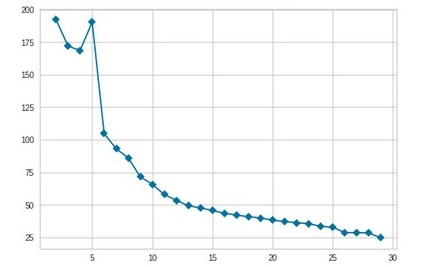
\includegraphics[width=8cm, height=5cm]{Images/Elbow.jpg} 
	\caption{Método Elbow }
	\label{fig:Elbow}
\end{figure}

\subsection{El método del Coeficiente Silhouette}
Partiendo de la metodología el coeficiente Silhoutte de una entidad es 1 si pertenece al clúster indicado. En otras palabras, a mayor valor global del coeficiente Silhoutte hace que la pertenencia de cada entidad al clúster determinado sea la mayor. En este caso particular se alcanza para k = 12. (ver Figura [ \ref*{fig:SCoe1} ])

\begin{figure}[h!]
	\centering
	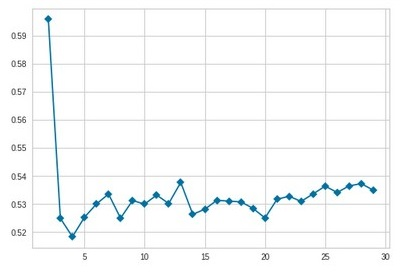
\includegraphics[width=8cm, height=5cm]{Images/SCoe1.jpg} 
	\caption{Método del Coeficiente Silhouette}
	\label{fig:SCoe1}
\end{figure}

\subsection{El método del Coeficiente Silhouette segunda variante}
La idea con esta segunda variante del método es más apreciativa. En la figura [ \ref{fig:SCoe2} ] se observa una línea roja discontinua, que marca el valor de compacidad para cada caso, si para algún k (número de clústeres iniciales), algún clúster (las figuras de colores) no alcanza el valor de compacidad ese k no debe ser escogido. Esta primera regla no se cumple en ninguno de los casos, por lo que se prosiguió a la siguiente regla en la metodología: escoger el k para el cuál las formas de los clústeres tengan la distribución más uniforme posible, o sea, que sus figuras sean similares. Como se puede apreciar en la figura [ \ref{fig:SCoe2} ], los clústeres más uniformes se alcanzan para K = 3.

\begin{figure}[h!]
	\centering
	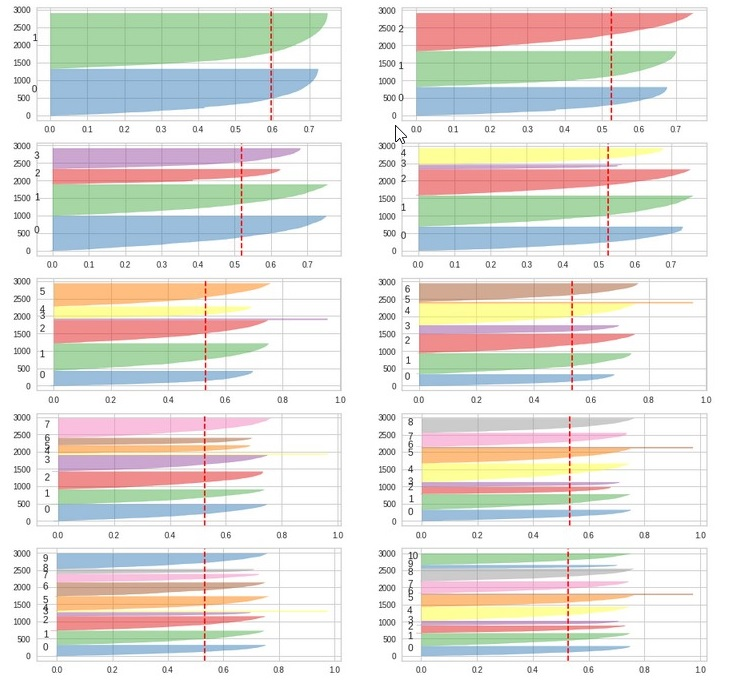
\includegraphics[width=8cm, height=10cm]{Images/SCoe2.jpg} 
	\caption{Método del Coeficiente Silhouette}
	\label{fig:SCoe2}
\end{figure}
\subsection{El método del índice Calinski-Harabasz}
Este algoritmo establece que a mayor valor del índice de Calinski-Harabasz es una mejor estimación para el número inicial de clústeres, ya que la misma garantiza una mayor compacidad de los clústeres. En este caso se seleccionó k = 29, como se observa en la figura [ \ref*{fig:CI} ], para 29 clústeres se alcanza el mayor valor para el índice de Calinski-Harabasz.


\begin{figure}[h!]
	\centering
	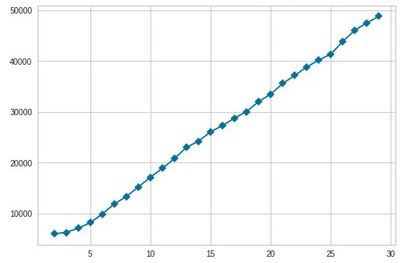
\includegraphics[width=8cm, height=5cm]{Images/CIndex.jpg} 
	\caption{Índice Calinski-Harabasz}
	\label{fig:CI}
\end{figure}
\subsection{El método del índice de Davies-Bouldin}
Este método tiene un principio muy similar al índice Calinski-Harabasz y al coeficiente Silhouette, dado que captura tanto la compacidad como la separación de los clústeres. A diferencia de ambos métodos mencionados a menor valor del índice de Davies-Bouldin, la literatura establece que se alcanzan mejores resultados. En este trabajo se seleccionó k = 12, dado que como se observa en la figura [ \ref{fig:DI} ], para 12 clústeres se alcanza el menor valor para el índice de Davies-Bouldin.

\begin{figure}[h!]
	\centering
	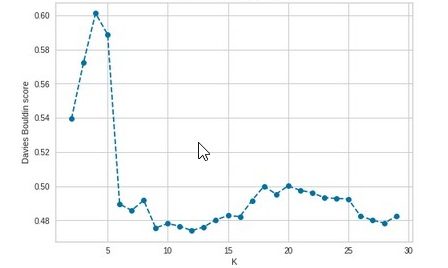
\includegraphics[width=8cm, height=5cm]{Images/DIndex.jpg} 
	\caption{Índice Davies-Bouldin}
	\label{fig:DI}
\end{figure}
\subsection{El método Dendrograma}
Dado que un dendrograma es una representación gráfica de datos en forma de árbol, dónde los datos se agrupan en subcategorías. En este método se toma el número de subcategorías como el número óptimo de clústeres, se obtuvo k = 3. Se puede apreciar en la figura [ \ref*{fig:Dend} ] donde cada categoría está marcada con un color solo aparecen tres colores, dictaminando que en el árbol de los datos analizados hay tres subcategorías presentes, o sea, que la mejor distribución de los datos sería en tres clústeres.

\begin{figure}[h!]
	\centering
	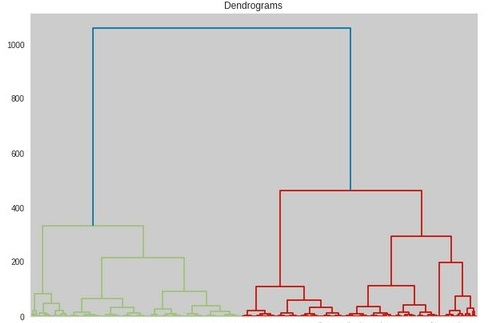
\includegraphics[width=8cm, height=6cm]{Images/Dendograma.jpg} 
	\caption{Método Dendrograma}
	\label{fig:Dend}
\end{figure}

\subsection{Resumen de los métodos}

\begin{table}[h!]
	 \begin{threeparttable}
	\begin{center}
		\begin{tabular}{| l | r | c |}
			\hline
			Método & K \tnote{1}  & Tiempo de Ejecución(Segundos) \\ \hline
			Gap en su versión estadística & 29 & 60 \\
			Elbow & 6 & 7 \\
			Coeficiente Silhouette & 13 & 11 \\
			Coeficiente Silhouette(2) & 3 & 6 \\
			Índice Calinski-Harabasz & 29 & 7 \\
			Índice de Davies-Bouldin & 12 & 6 \\
			Dendrograma & 3 & 14 \\
			Moda & 3 & -\\
			Promedio & 13 & - \\ \hline
		\end{tabular}
		\begin{tablenotes}
		\item[1] K : Representa el número de clústeres óptimo para Kmeans.
		
		\end{tablenotes}  
		\caption{Número de Clústeres Óptimo vs Tiempo de Ejecución}
		\label{tab:resumenMetodos}
	\end{center}
	 \end{threeparttable}
\end{table}



\begin{figure}[h!]
	\centering
	
	\begin{subfigure}[b]{0.49\linewidth}
		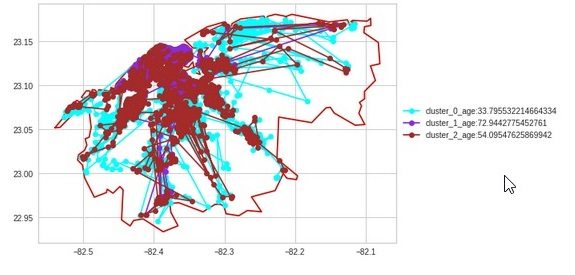
\includegraphics[width=\linewidth, height=3cm]{Images/3.jpg}
		\caption{Kmeans tres Clústeres}
	\end{subfigure}
	\begin{subfigure}[b]{0.49\linewidth}
		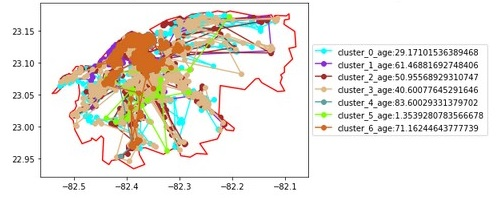
\includegraphics[width=\linewidth, height=3cm]{Images/6.jpg}
		\caption{Kmeans seis Clústeres}
	\end{subfigure}
	\begin{subfigure}[b]{0.49\linewidth}
		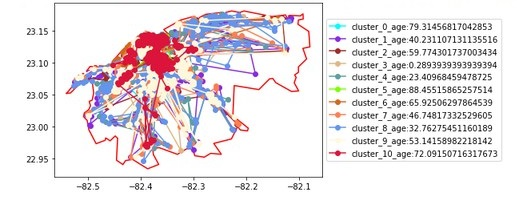
\includegraphics[width=\linewidth, height=3cm]{Images/11.jpg}
		\caption{Kmeans 11 Clústeres}
	\end{subfigure}
	\begin{subfigure}[b]{0.49\linewidth}
		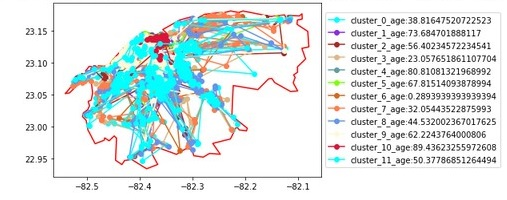
\includegraphics[width=\linewidth, height=3cm]{Images/12.jpg}
		\caption{Kmeans 12 Clústeres}
	\end{subfigure}
	\begin{subfigure}[b]{0.49\linewidth}
		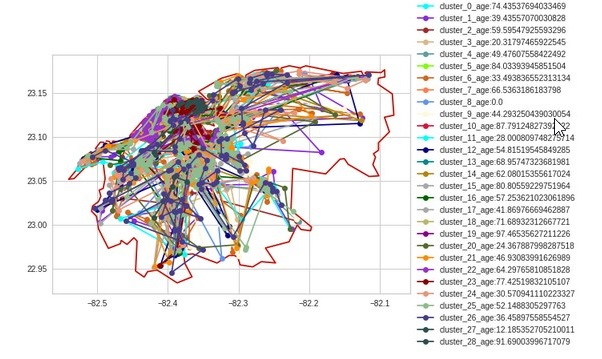
\includegraphics[width=\linewidth, height=3cm]{Images/29.jpg}
		\caption{Kmeans 29 Clústeres}
	\end{subfigure}
	\caption{Distribución de la Habana según Kmeans}
	\label{fig:Kmeans}
\end{figure}

El análisis realizado se identificó K = 3 como el número de clústeres óptimo para el algoritmo de Kmeans, para el conjunto de datos estudiados. Por un lado, es el valor de la moda de todos los algoritmos estudiados para la estimación de dicho parámetro y por otro resultó ser el más descriptivo en cuanto a las diferencias de los clústeres. Esto se puede apreciar claramente en las imágenes asociadas a cada uno de los resultados de los métodos donde a mayor número de clústeres menor las diferencias entre el valor de su centroide, lo que impedía tomar decisiones certeras. La figura [ \ref{fig:Conc} ], muestra el resultado final de aplicar el algoritmo k means con k =3 y el valor de sus centroides.

\begin{figure}[h!]
	\centering
	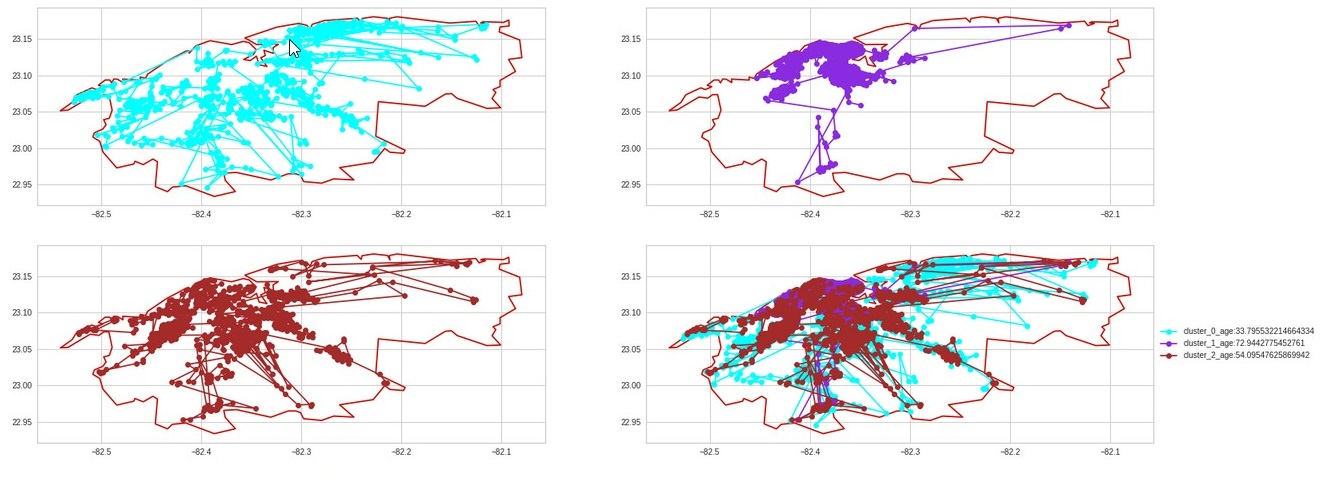
\includegraphics[width=15cm, height=7cm]{Images/Conclusion.jpg} 
	\caption{Habana dividida en tres clústeres}
	\label{fig:Conc}
\end{figure}

En muchas ocasiones un análisis desde lo local, es fundamental en el estudio de una problemática. El estudio de la segregación en la habana con respecto a su casco urbanístico no es la excepción. Existen municipios que se comportan como la ciudad que ya de por si marca un envejecimiento de las viviendas preocupante mientras que existen otros como es el caso de la Habana Vieja que sus promedios de edades son muy superiores a la media. Sin embargo, para la periferia de la ciudad municipios como el Cotorro o Boyeros son realmente “jóvenes” si de antigüedad de sus viviendas se trata.




\begin{figure}[h!]
	\centering
	\begin{subfigure}[b]{0.49\linewidth}
		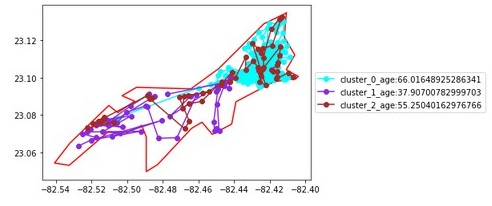
\includegraphics[width=\linewidth, height=3cm]{Images/Playa.jpg}
		\caption{Playa}
	\end{subfigure}
	\begin{subfigure}[b]{0.49\linewidth}
		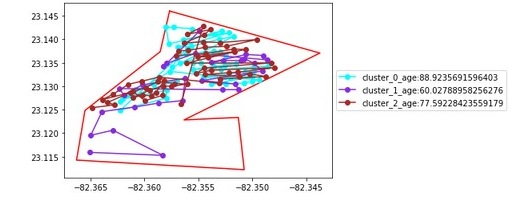
\includegraphics[width=\linewidth, height=3cm]{Images/HabV.jpg}
		\caption{Habana Vieja}
	\end{subfigure}
	\begin{subfigure}[b]{0.49\linewidth}
		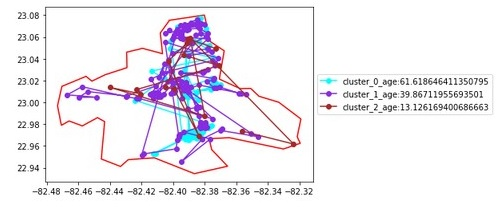
\includegraphics[width=\linewidth, height=3cm]{Images/Boyeros.jpg}
		\caption{Boyeros}
	\end{subfigure}
	\caption{Municipios de la Habana}
	\label{fig:muns}
	
\end{figure}

Los clústeres obtenidos para el resto de los municipios pueden consultarse en el Anexo [ \ref{chapter:Anexo} ].

\newpage
Queda propuesto para trabajos posteriores realizar un análisis más profundo a nivel de localidad para los distintos municipios de la Habana. Estudio futuro que espera aportar nuevos y determinantes argumentos para establecer una comparación más a fondo entre lo local y lo global(municipio-ciudad).
\newpage
\section{Experimento 2: Trayectorias Simples – Trayectorias simples modificadas}
Los resultados de ambas metodologías para los datos de la proporción de las viviendas de antes del 1959 con respecto al total de viviendas en la Habana, se compararon en cuanto al tiempo de ejecución y el recorrido descrito sobre el mapa.

\begin{table}[h!]
	\begin{center}
		\begin{tabular}{| l | c | c |}
			\hline
			Método & Una Trayectoria & Todas las Trayectorias \\ \hline
			Trayectorias Simples & - & - \\
			Trayectorias simples modificadas & - & - \\ \hline
		
		\end{tabular}
		\caption{Tiempo de Ejecución de las Trayectorias}
		\label{tab:resumenTrayectorias}
	\end{center}
\end{table}

\begin{figure}[h!]
	\centering
	\begin{subfigure}[b]{0.49\linewidth}
		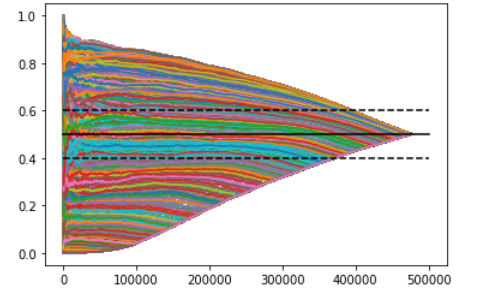
\includegraphics[width=\linewidth, height=3cm]{Images/TrayecCon.png}
		\caption{Trayectorias Modificadas}
	\end{subfigure}
	\begin{subfigure}[b]{0.49\linewidth}
		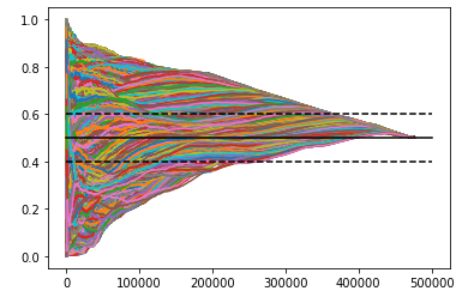
\includegraphics[width=\linewidth, height=3cm]{Images/ValueTray.png}
		\caption{Trayectorias Simples}
	\end{subfigure}

	\caption{Trayectorias de la Habana}
	\label{fig:trayectorias}
\end{figure}

La imagen [ \ref{fig:trayectorias} ] describen el conjunto de todas las trayectorias para ambas metodologías. Las fluctuaciones en las figuras determinan qué tan rápido convergen las trayectorias.

\newpage

Un análisis desde lo local puede resultar mucho más provechoso para analizar las diferencias entre ambos métodos de trayectorias. Las figura [ \ref{fig:Onetrayectorias} ] muestran el comportamiento de una única trayectoria, que parte desde el mismo distrito utilizando ambos métodos de trayectorias. En la figura [ \ref{fig:OnetrayectoriasM} ] se muestra una convergencia más lineal pues el recorrido en orden del valor de la variable. En la figura [ \ref{fig:OnetrayectoriasS} ] se muestra una convergencia menos lineal esto se debe a que el recorrido se realiza por cercanía lo que implica que varía grandemente el valor que toma la variable de estudio independientemente de la cercanía.

\begin{figure}[h!]
	\centering
	\begin{subfigure}[b]{0.49\linewidth}
		\includegraphics[width=\linewidth, height=3cm]{Images/OneTrayecV.png}
		\caption{Trayectorias Modificadas}
		\label{fig:OnetrayectoriasM}
	\end{subfigure}
	\begin{subfigure}[b]{0.49\linewidth}
		\includegraphics[width=\linewidth, height=3cm]{Images/OneTrayecD.png}
		\caption{Trayectorias Simples}
		\label{fig:OnetrayectoriasS}
	\end{subfigure}
	
	\caption{Única Trayectoria}
	\label{fig:Onetrayectorias}
\end{figure}

\subsection{Recorrido en el mapa }

\begin{figure}[h!]
	\centering
	\begin{subfigure}[b]{0.49\linewidth}
		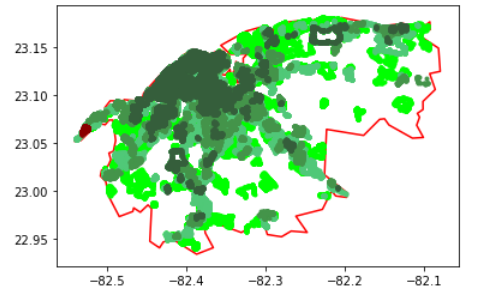
\includegraphics[width=\linewidth, height=3cm]{Images/TrayecVa.png}
		\caption{Trayectorias Modificadas}
		\label{fig:TrayecVa}
	\end{subfigure}
	\begin{subfigure}[b]{0.49\linewidth}
		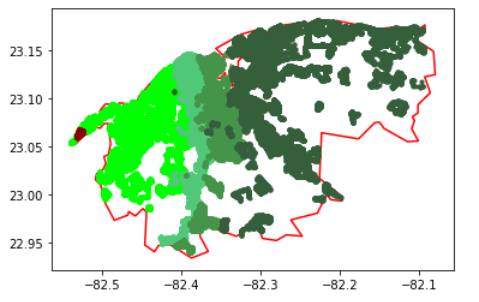
\includegraphics[width=\linewidth, height=3cm]{Images/TrayecDis.png}
		\caption{Trayectorias Simples}
		\label{fig:TrayecDis}
	\end{subfigure}
	
	\caption{Recorrido por el mapa}
	\label{fig:RecorridoTrayectorias}
\end{figure}

La figura [ \ref{fig:RecorridoTrayectorias} ]  muestran el recorrido en el mapa para ambas metodologías. El método de trayectorias simples muestra un recorrido claramente por distancia geográfica entre distritos [ \ref{fig:TrayecDis} ], mientras que el método de trayectorias modificadas [ \ref{fig:TrayecVa} ] hace un recorrido desde la periferia hasta el interior. Este comportamiento del recorrido del método de trayectorias modificadas, se debe en gran medida al distrito seleccionado. En este caso se seleccionó un distrito de la periferia, marcado con un punto rojo, se puede observar como la trayectoria primero recorre la periferia de la ciudad y luego se va adentrando en la misma. El orden del recorrido está dado por el grado de intensidad del color verde, mientras más oscuro más tarde se recorrió. Lo que ratifica que los municipios de la periferia tienen edificaciones más jóvenes.

\section{Experimento 3: Comparación Kmeans – Trajectorias Simples Modificado}
El objetivo principal de esta comparación es analizar la distribución realizada por ambos algoritmos a los distritos de la Habana. Para ello un punto inicial es lograr obtener a partir del método de trayectorias el número de clústeres óptimo(K) para Kmeans. El método propuesto para realizar dicha tarea, propone una estimación del K a partir del momento de entrada al intervalo de confianza de cada trayectoria.

\begin{figure}[h!]
	\centering
	\begin{subfigure}[b]{0.6\linewidth}
		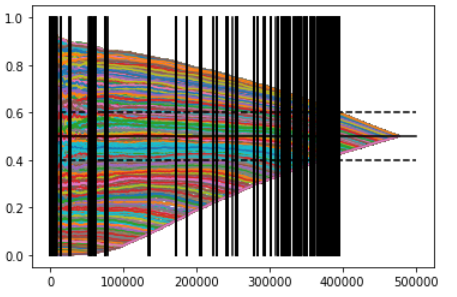
\includegraphics[width=\linewidth, height=5cm]{Images/Convergency2.png}
		\caption{Trayectorias Modificadas Convergencia}
		\label{fig:Convergency2}
	\end{subfigure}
	\begin{subfigure}[b]{0.6\linewidth}
		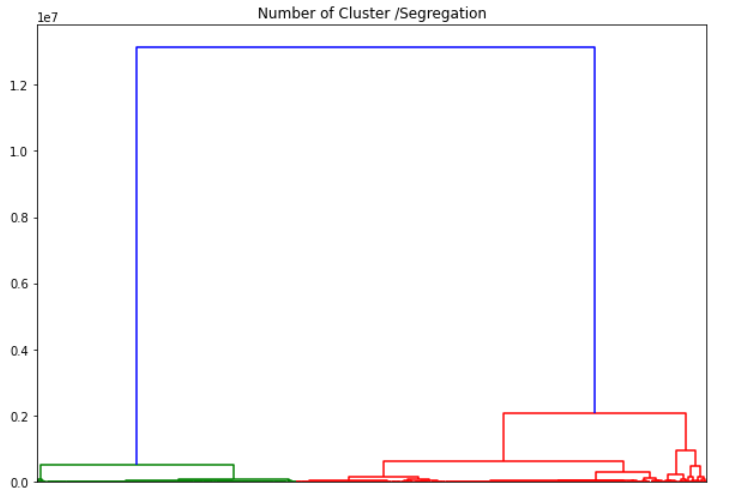
\includegraphics[width=\linewidth, height=5cm]{Images/ConvergenciaTrayec.png}
		\caption{Dendograma de Convergencias}
		\label{fig:ConvergenciaTrayec}
	\end{subfigure}
	
	\caption{Convergencia de Trayectorias}
	\label{fig:TrayectoriasConV}
\end{figure}

Como se puede apreciar en la figura [ \ref{fig:TrayectoriasConV} ] el resultado del método propuesto fue k = 3. La entrada del método fueron los datos de la proporción de las viviendas de antes del 1959 con respecto al total de viviendas en la Habana. El resultado corrobora la elección realizada en el primer experimento.

En este punto se hace necesaria la siguiente interrogante: \textbf{¿Si ambos métodos dividen la ciudad en tres clústeres, son acaso los mismos?}

\begin{figure}[h!]
	\centering
	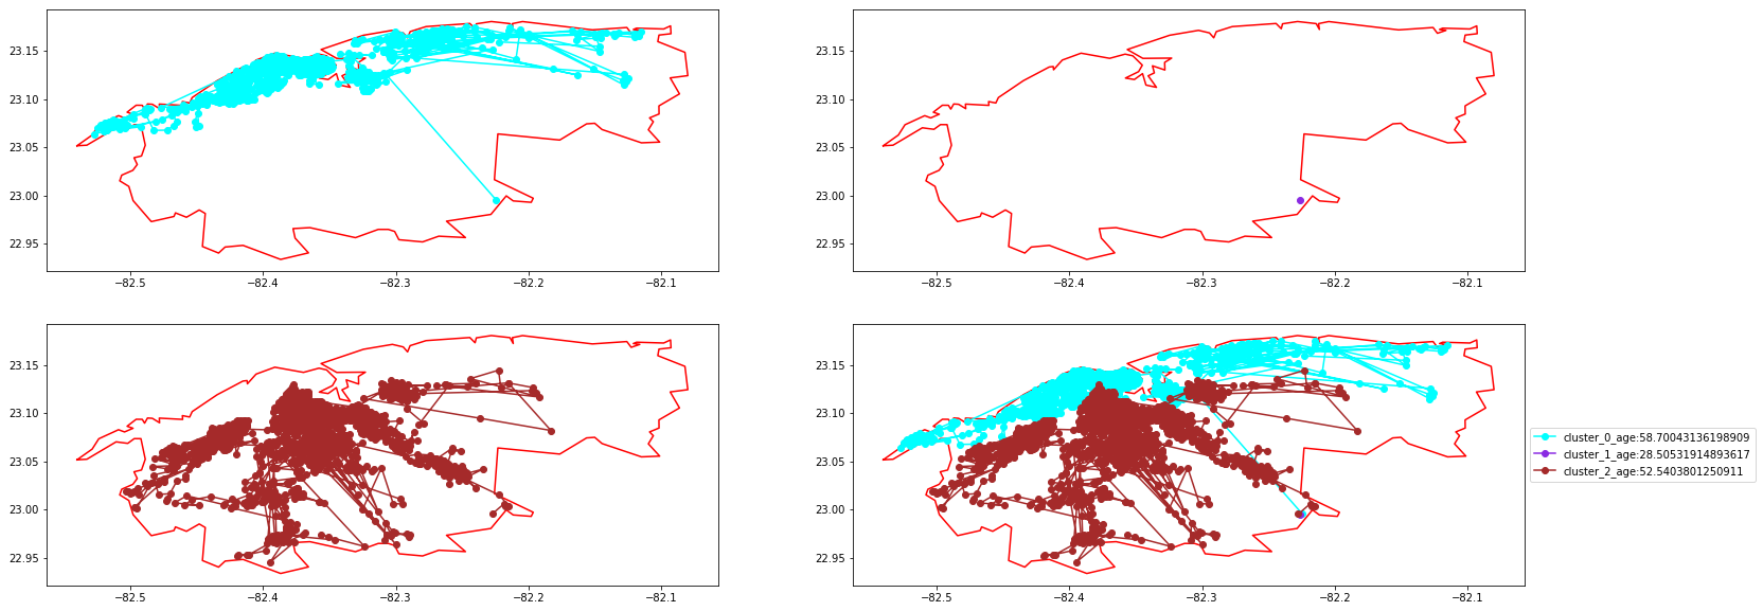
\includegraphics[width=15cm, height=7cm]{Images/Hab3KTrayec.png}
	\caption{Habana dividida por el método de trayectorias}
	\label{fig:Hab3KTrayec}
\end{figure}

La división de la Habana que realizó el algoritmo de trayectorias simples describe dos clústeres bien definidos y un punto aislado. La Imagen [ \ref{fig:Hab3KTrayec} ] muestra una clara separación entre las áreas, no obstante, el promedio de edad de los dos clústeres grandes no difiere tanto. Esto podría indicar que no existe segregación, sin embargo, ocurre todo lo contrario. Sucede que los distritos de la zona norte de la Habana, marcados con un color azul en la figura [ \ref{fig:Hab3KTrayec} ], son más antiguos por lo tanto son más semejantes a la Ciudad lo que implica que tienen una convergencia rápida. En cambio, los distritos de la parte sur de la ciudad, marcados con carmelita en la figura [ \ref{fig:Hab3KTrayec} ], son más jóvenes y por tanto demoran más en converger a la media de la ciudad. Kmeans describe una ciudad muy compacta con tres clústeres completamente entrelazados en la figura [ \ref{fig:Conc} ]. Un detalle importante a destacar en algoritmo de Kmeans es la clara diferencia de edad de los centroides de los clústeres que permite llegar a conclusiones más certeras en cuanto a la segregación.

\begin{table}[h!]
	\begin{center}
		\begin{tabular}{| l | c | c |}
			\hline
			Algotirmo & Cantidad de Grupos & Tiempo de Ejecución(Seg) \\ \hline
			Kmeas & 3 & - \\
			Trayectorias Simples Modificadas & 3 & - \\ \hline
			
		\end{tabular}
		\caption{Kmeans vs Trayectorias Simples Modificadas}
		\label{tab:comparacionMetodos}
	\end{center}
\end{table}

Ambos algoritmos describen la segregación residencial, pero de forma diferente. Kmeans ofrece una mirada global al problema de la segregación agrupando a los distritos en sectores no necesariamente aislados, pero si con características diferentes entre ellos. Kmeas evidencia que la Habana es una ciudad envejecida en su centro, si tomamos como centro el origen de los asentamientos de la ciudad y relativamente joven en la periferia de la misma. El algoritmo de Trayectorias modificadas permite abordar conclusiones semejantes a las ofrecidas por Kmenas, sin embargo, resulta más efectivo en cuanto al análisis desde lo local en una comparación con lo global. Cuán rápido converge un distrito, o sea, entra en el intervalo de confianza para el valor evaluado en la trayectoria, es una herramienta fundamental para determinar la existencia de segregación en el mismo.
